%%%%%%%%%%%% DISEÑO Y DESARROLLO / DESIGN & IMPLEMENTATION CHAPTER %%%%%%%%%%%%%%%%%%%%%%%%%%%%%%%%%%%%%%%%%%%
\chapter{Experiments and Results}
\label{cha:experiments}

This chapter presents a series of practical experiments aimed at exploring the potential of utilizing DAAM and the proposed extensions for object segmentation in synthetically generated images, particularly focusing on urban scenes. To conduct these experiments, a synthetic dataset was created using Stable Diffusion as the foundational model (Sec. \ref{sec:experiment-framework}). The experiments are organized into three sections, mirroring the structure of the proposed methods proposed in Chapter \ref{cha:methodology}, in order to assess the impact of each modification.

The first section, \ref{sec:experiment-daam}, evaluates the masks generated by DAAM in its original formulation \cite{DAAM} to establish a baseline for comparing the proposed modifications. Next, in section \ref{sec:experiment-daam-ov}, we measure the effects of linearizing the attention maps using Linear DAAMs (Sec. \ref{cha:methodology-ov-daam}). In section \ref{sec:experiment-optimization}, we optimize text prompts for each class in the dataset and repeat the evaluation. Finally, in Section \ref{sec:experiment-summary}, we provide a summary of the experiment and a comparison of the results.

The goal of these experiments is to analyze the limitations and potential benefits of utilizing internally generated attentions from an LDM within a simplified urban scene scenario. Additionally, we aim to identify possible directions for future research, expanding the application of DAAM beyond its initial framework.

\section{Experiment framework}
\label{sec:experiment-framework}

This section overviews the experiment framework, including the architecture used and the details of the generated dataset.

To conduct the experiments, a synthetic dataset of simple urban scene scenarios was created. The dataset was intentionally designed to emphasize simplicity, with each image featuring a single primary object class. Four commonly encountered classes \cite{Cityscapes} in urban scene semantic segmentation tasks were chosen: ``car,'' ``person,'' ``traffic light,'' and ``rider''.

The images were generated using the Stable Diffusion (2-base) architecture, which was also employed in the original DAAM paper \cite{DAAM}. However, the proposed methods and implementation are compatible with other versions of Stable Diffusion \cite{rombach2022high}. Initial tests conducted with other versions have yielded similar results.

 A dataset consisting of 200 images was created, with 50 images per class. The text prompt ``A \textlangle token\textrangle\ in an urban environment'' was utilized to generate the images, where the token corresponds to each class name. In order to generate diverse images with the same text prompt, the random seed used to generate the initial noisy latent vector was changed for each image. For more detailed information about the dataset and to access the images, please refer to Appendix \ref{chap:appendix-text-dataset}.
 
The LDM noise modeling process employs the PNDM scheduler \cite{liu2022pseudo}, which utilizes a multi-step Runge-Kutta method to model the diffusion process as an ODE and accelerate the convergence of the diffusion process. The reverse diffusion model uses 30 timesteps to generate the images. To ensure reproducibility, the random seeds used in the process were stored, allowing for the replication of the diffusion process and generation of the same images and internal attentions.



\begin{figure}
\centering
  % First column
  \begin{subfigure}{0.24\columnwidth}
   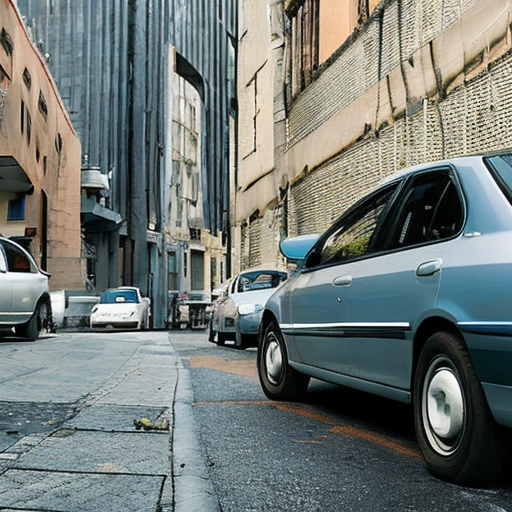
\includegraphics[width=\columnwidth]{img/4-experiments/dataset_example_car.png}
   \caption{Car}
   \label{subfig:dataset-example-car}
  \end{subfigure}
  \begin{subfigure}{0.24\columnwidth}
   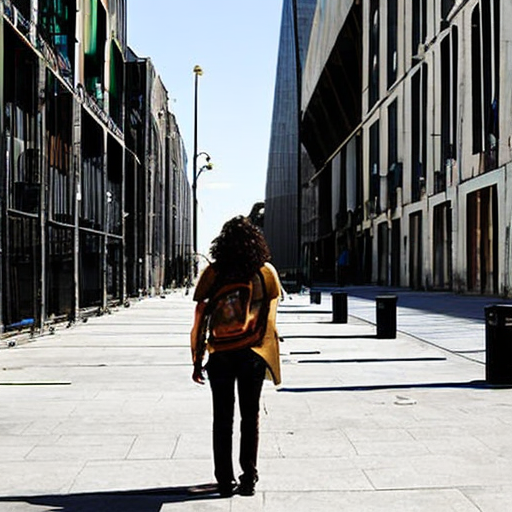
\includegraphics[width=\columnwidth]{img/4-experiments/dataset_example_person.png}
   \caption{Person}
   \label{subfig:dataset-example-person}
  \end{subfigure}
  \begin{subfigure}{0.24\columnwidth}
   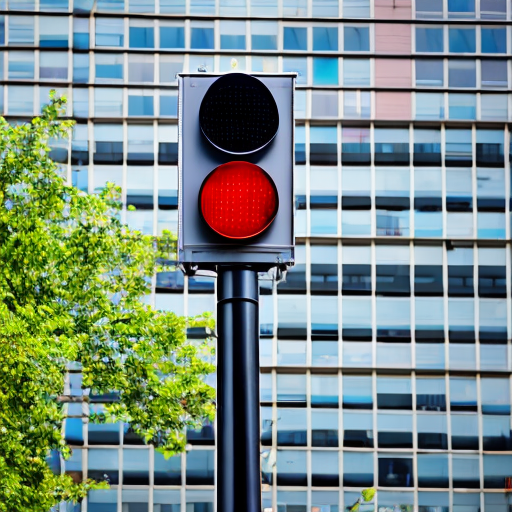
\includegraphics[width=\columnwidth]{img/4-experiments/dataset_example_traffic light.png}
   \caption{Traffic Light}
   \label{subfig:dataset-example-traffic}
  \end{subfigure}
  \begin{subfigure}{0.24\columnwidth}
   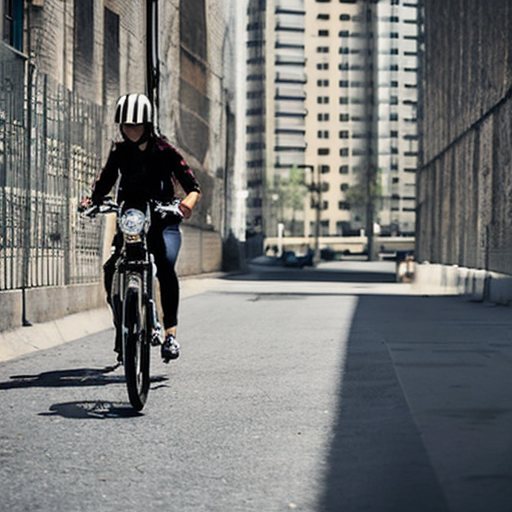
\includegraphics[width=\columnwidth]{img/4-experiments/dataset_example_rider.png}
   \caption{Rider}
   \label{subfig:dataset-example-rider}
  \end{subfigure}
  \par\bigskip
  \begin{subfigure}{0.24\columnwidth}
   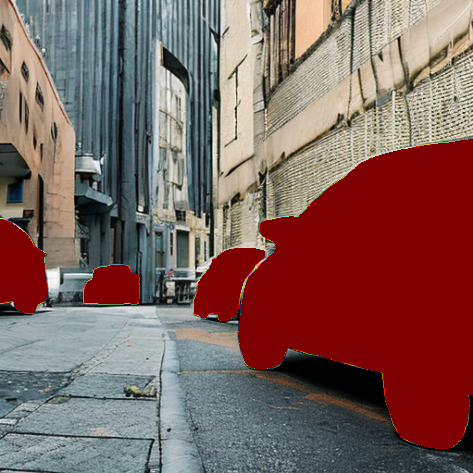
\includegraphics[width=\columnwidth]{img/4-experiments/example_mask_car.png}
   \caption{Car mask}
   \label{subfig:dataset-example-car-mask}
  \end{subfigure}
  \begin{subfigure}{0.24\columnwidth}
   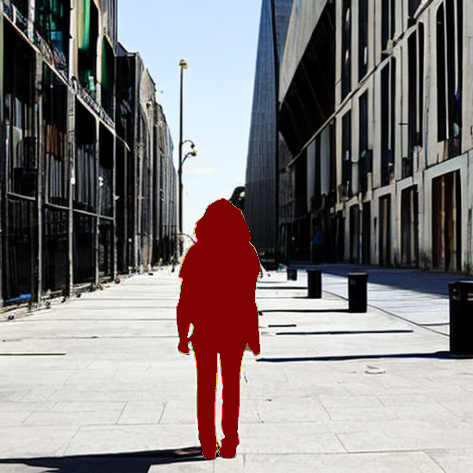
\includegraphics[width=\columnwidth]{img/4-experiments/example_mask_person.png}
   \caption{Person mask}
   \label{subfig:dataset-example-person-mask}
  \end{subfigure}
  \begin{subfigure}{0.24\columnwidth}
   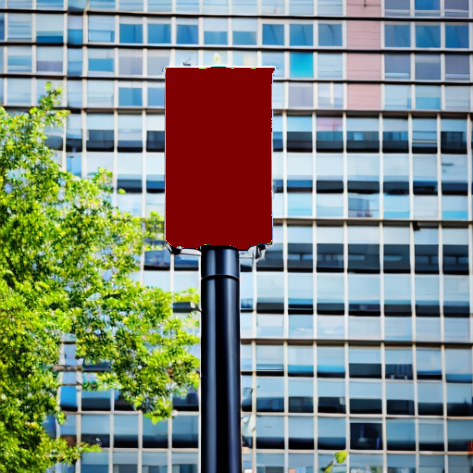
\includegraphics[width=\columnwidth]{img/4-experiments/example_mask_traffic light.png}
   \caption{Traffic light mask}
   \label{subfig:dataset-example-traffic-mask}
  \end{subfigure}
    \begin{subfigure}{0.24\columnwidth}
   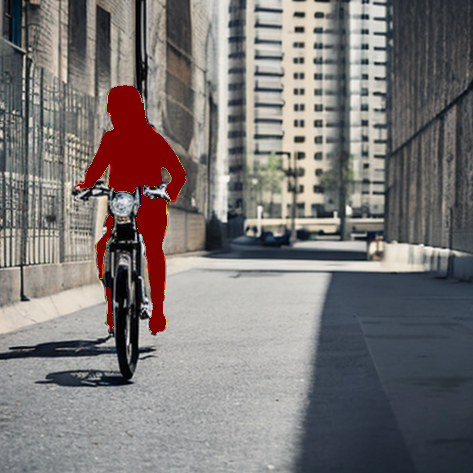
\includegraphics[width=\columnwidth]{img/4-experiments/example_mask_rider.png}
   \caption{Rider mask}
   \label{subfig:dataset-example-rider-mask}
  \end{subfigure}
  \caption[Synthetic dataset examples]{Visual examples of images and corresponding segmentation masks in the dataset. The first row showcases four distinct scenes, each representing one of the classes: ``car'', ``person'', ``traffic light'', and ``rider''. In the second row, the same images are presented with their respective ground truths overlayed.}
  \label{fig:dataset-examples}
  \end{figure}
  
Figure \ref{fig:dataset-examples} showcases an example image for each of the four classes in the dataset (Figs. \ref{subfig:dataset-example-car} to \ref{subfig:dataset-example-rider}). The images illustrate the simplicity of the scenes, with a clear focus on a single primary object from each class.

Ground truth annotations were created for each of the 200 images based on their corresponding primary class, following the standards used in Cityscapes \cite{Cityscapes}. The SAM (Segment Anything Model) \cite{SAM} was employed to generate accurate segmentation masks, with manual supervision to ensure precise annotations. These segmentation masks serve as the reference for measuring the Intersection over Union (IoU) between the binary heatmaps generated by DAAM and its proposed extensions.

The latent space dimensions of Stable Diffusion 2-base (referred to as $w \times h$ in Chapter \ref{cha:methodology}), and therefore the dimensions of the generated attention maps, are 64 x 64. However, the images are generated at a resolution of 512 x 512, due to the VAE final step \cite{rombach2022high}. To measure the IoU, the heatmaps are rescaled using bicubic interpolation to match the size of the images.


Examples of the binary masks can be seen in Figs. \ref{subfig:dataset-example-car-mask} to \ref{subfig:dataset-example-rider-mask}. Notably, for the traffic light class (\ref{subfig:dataset-example-traffic-mask}), the post is excluded, as it is typically labeled as class ``pole'' in urban scene segmentation datasets. Similarly, the rider class includes only the person riding the motorcycle, without including the motorcycle itself (\ref{subfig:dataset-example-rider-mask}).




\section{DAAM baseline}
\label{sec:experiment-daam}

\begin{figure}
\centering
  % First column
  \begin{subfigure}{0.24\columnwidth}
   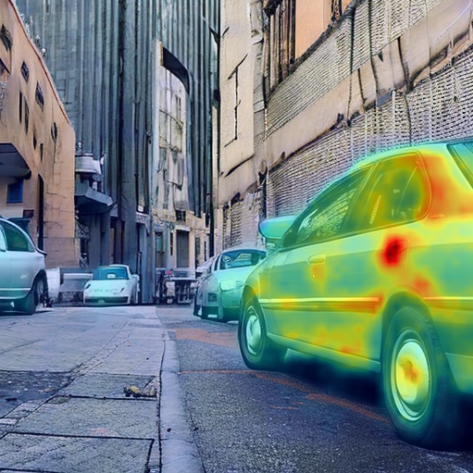
\includegraphics[width=\columnwidth]{img/4-experiments/dataset_example_daam_heatmap_car.png}
   \caption{Car}
   \label{subfig:dataset-example-car-daam}
  \end{subfigure}
  \begin{subfigure}{0.24\columnwidth}
   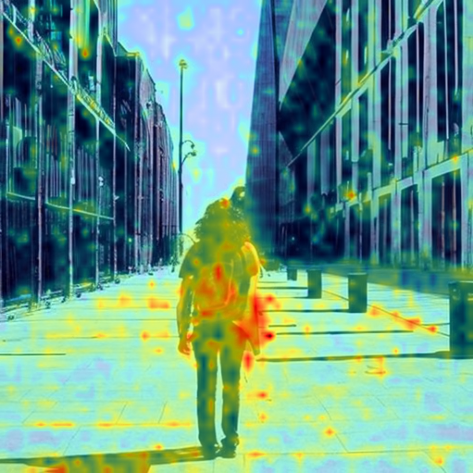
\includegraphics[width=\columnwidth]{img/4-experiments/dataset_example_daam_heatmap_person.png}
   \caption{Person}
   \label{subfig:dataset-example-person-daam}
  \end{subfigure}
  \begin{subfigure}{0.24\columnwidth}
   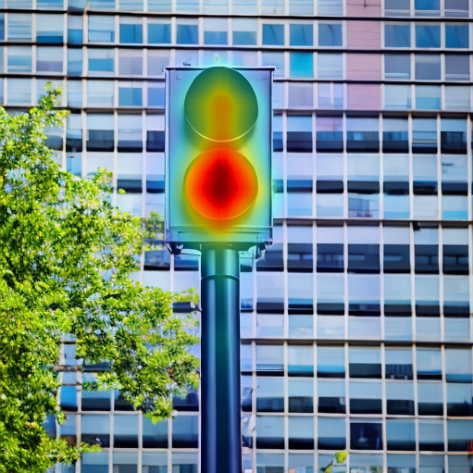
\includegraphics[width=\columnwidth]{img/4-experiments/dataset_example_daam_heatmap_traffic light.png}
   \caption{Traffic light}
   \label{subfig:dataset-example-traffic-daam}
  \end{subfigure}
  \begin{subfigure}{0.24\columnwidth}
   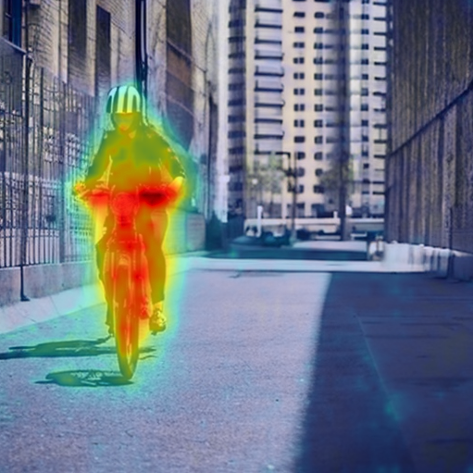
\includegraphics[width=\columnwidth]{img/4-experiments/dataset_example_daam_heatmap_rider.png}
   \caption{Rider}
   \label{subfig:dataset-example-rider-daam}
  \end{subfigure}
  \caption[Examples of DAAM-generated soft heatmaps]{Examples of DAAM-generated soft heatmaps. Each subfigure displays an image for each class with the overlayed soft heatmap generated using DAAM.}
  \label{fig:dataset-examples-daam}
  \end{figure}

In this initial experiment, we evaluate the masks generated by the original DAAM method \cite{DAAM}. These findings establish a baseline for understanding the performance of DAAM's attention in semantic segmentation tasks and identifying the key challenges that arise when using this explainability technique in such contexts.

To evaluate the masks, we generated soft heatmaps, $D^{\mathbb{R}}_k$, following Eq. \ref{eq:daam-summing}, using the original implementation of DAAM. The token corresponding to the class name was extracted from the text prompt ``A \textlangle token\textrangle\ in an urban environment'' for each class, except for the ``traffic light'' class, which consisted of two tokens. To prevent attention from being dispersed throughout the entire scene due to the semantic association with the word ``traffic,'' we specifically considered the token ``light'' for this class.

Figure \ref{fig:dataset-examples-daam} displays the soft heatmaps for each example image of the four classes. We observe distinct issues in each class, which can be explained from a semantic perspective of the generated attention:

\begin{itemize}
\item In the example of the ``car'' class (Fig. \ref{subfig:dataset-example-car-daam}), the attention attributed to the word ``car'' correctly focuses on the cars. However, the attention within these cars is irregular, and in this specific example, there is minimal attention given to the cars in the background of the scene.
\item For the ``person'' class (Fig. \ref{subfig:dataset-example-person-daam}), the attention is dispersed throughout the image, as the semantic relationship learned by the network for the word ``person'' influences the entire scene.
\item In the ``traffic light'' class (Fig. \ref{subfig:dataset-example-traffic-daam}), where we considered the attention generated by the word ``light,'' the attention correctly focuses on the red light of the traffic signal (see Fig. \ref{subfig:dataset-example-traffic}). However, the segmentation does not cover the entire expected area according to the annotation criteria (\ref{subfig:dataset-example-traffic-mask}).
\item For the ``rider'' class (Fig. \ref{subfig:dataset-example-rider-daam}), the attention is primarily concentrated on the motorcycle. This could be interpreted as the network learning that the presence of a motorcycle gives semantic meaning to the concept rider. However, our goal is to obtain a mask that specifically segments the person riding the motorcycle.
\end{itemize}

\begin{figure}
    \centering
    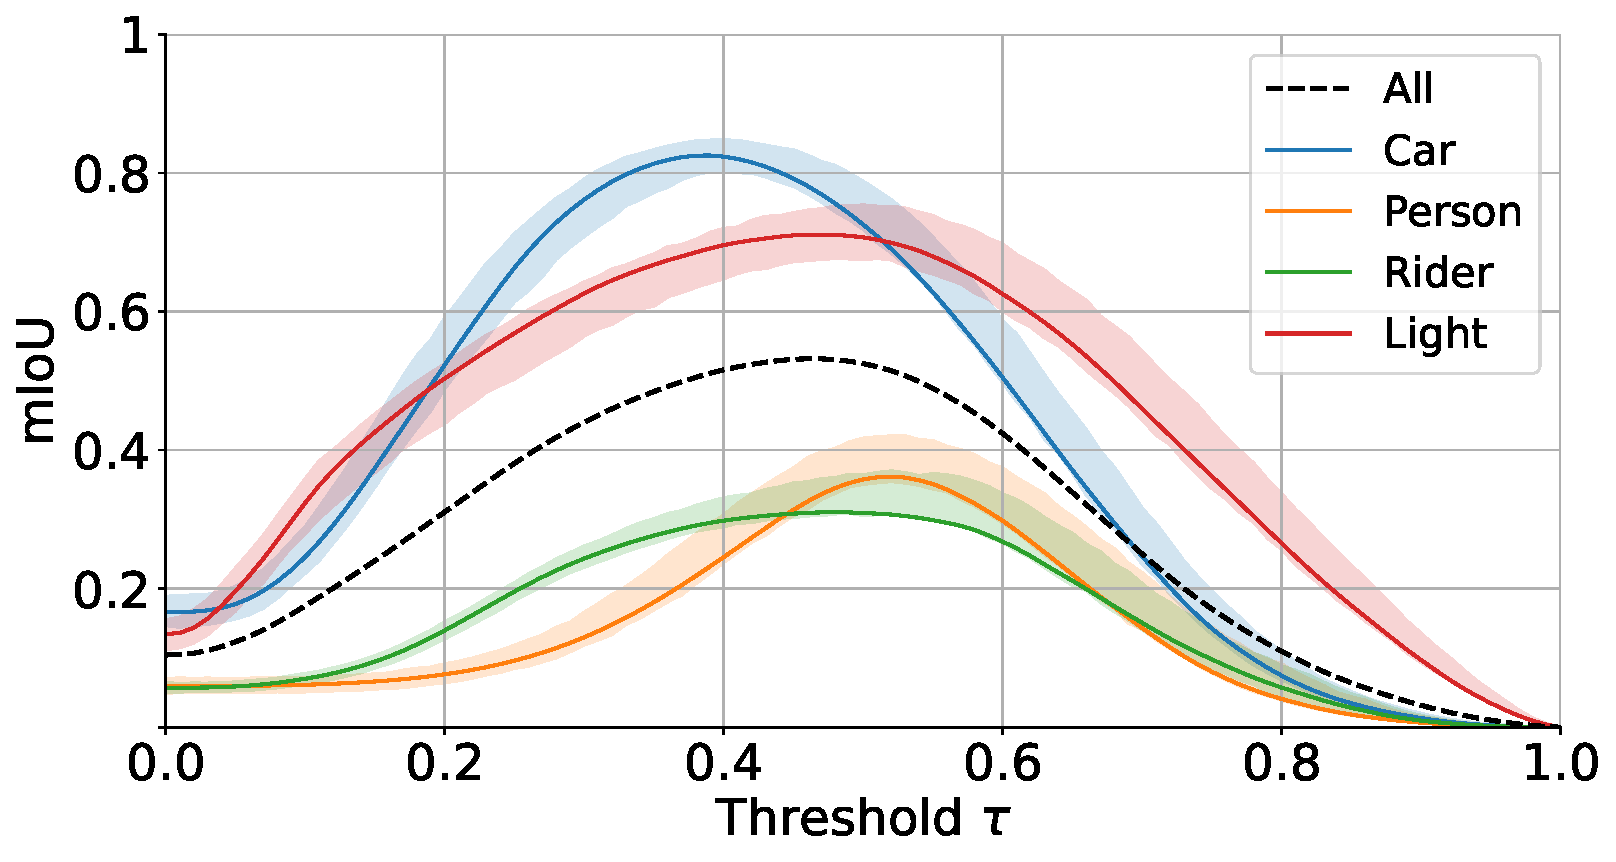
\includegraphics[width=1\columnwidth]{img/4-experiments/daam-threshold-iou-experiment-min-max.pdf}
    \caption[Comparison of mIoU per class using DAAM]{Comparison of mean Intersection over Union (mIoU) for each class at different threshold values. The graph illustrates the mIoU values for the ``car,'' ``light,'' ``person,'' and ``rider'' classes, along with the 5th and 95th percentile values. The curves demonstrate distinct profiles for each class, highlighting the varying performance of DAAM in segmenting different object classes.}
    \label{fig:miou-class-curves}
\end{figure}


To assess the performance in terms of mIoU, we employed a fixed threshold to binarize the heatmaps (as per Eq. \ref{eq:daam-binary}). Considering that mIoU is dependent on the threshold, we varied it from 0 to 1 to examine the curves' behavior. The results of the experiment are shown in Figure \ref{fig:miou-class-curves}, revealing four distinct patterns for each class. The figure showcases the mIoU (per-pixel) for each class and includes the 5th and 95th percentile mIoU values for individual class examples. It is noteworthy that the behavior of mIoU across different thresholds remains consistent within each class. The curves' profiles can be explained by the challenges illustrated in the previous examples, which are prevalent throughout the dataset:

\begin{itemize}
\item The ``car'' class is segmented correctly, reaching a maximun mIoU of 82.5.
\item The ``light'' class achieves an mIoU of 71.1, as the attention generated only relates to the light part of the traffic light.
\item The ``person'' class reaches an mIoU of 36.2, as the attention is centered on the persons' silhouettes but generates dispersed attention throughout the scenes.
\item The ``rider'' class has a maximum IoU of 31.0 because the network's concept aligns with the object ``motorcycle'' rather than the rider.
\end{itemize}

These results underscore the limitations of utilizing DAAM as a direct means of extracting ground truth, even in a straightforward scenario. The challenge lies in effectively controlling the attention's focus, which is constrained by the choice of words in the prompt used to generate the image. In the subsequent experiments, we examine this same scenario using the proposed modifications of the method, aiming to extend its applicability beyond its original purpose of explainability.


\section{Linear Open Vocabulary DAAM}
\label{sec:experiment-daam-ov}


\begin{figure}
\centering
  % First column
  \begin{subfigure}{0.24\columnwidth}
   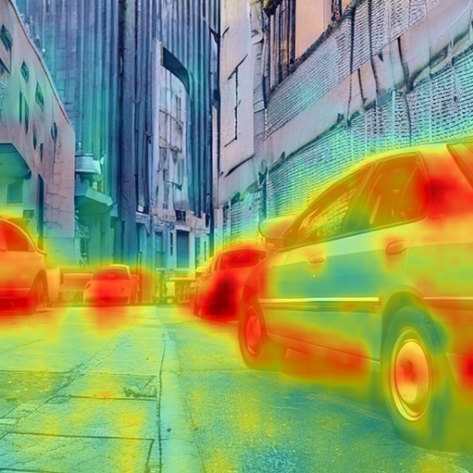
\includegraphics[width=\columnwidth]{img/4-experiments/example-linear-daam-overlay-car.png}
   \caption{Car}
   \label{subfig:dataset-example-car-daam-linear}
  \end{subfigure}
  \begin{subfigure}{0.24\columnwidth}
   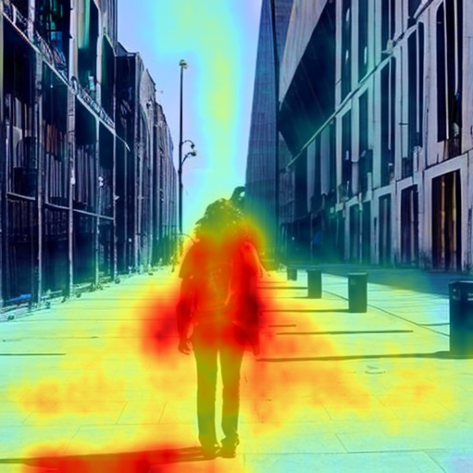
\includegraphics[width=\columnwidth]{img/4-experiments/example-linear-daam-overlay-person.png}
   \caption{Person}
   \label{subfig:dataset-example-person-daam-linear}
  \end{subfigure}
  \begin{subfigure}{0.24\columnwidth}
   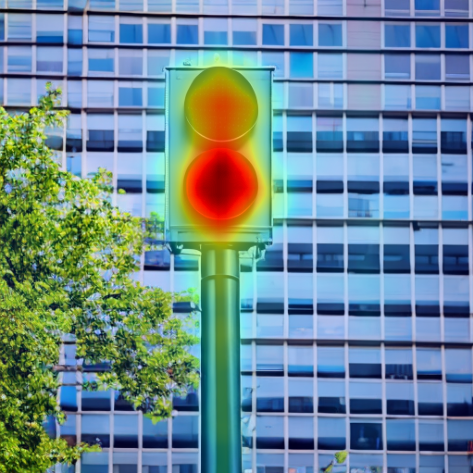
\includegraphics[width=\columnwidth]{img/4-experiments/example-linear-daam-overlay-traffic light.png}
   \caption{Traffic light}
   \label{subfig:dataset-example-traffic-daam-linear}
  \end{subfigure}
  \begin{subfigure}{0.24\columnwidth}
   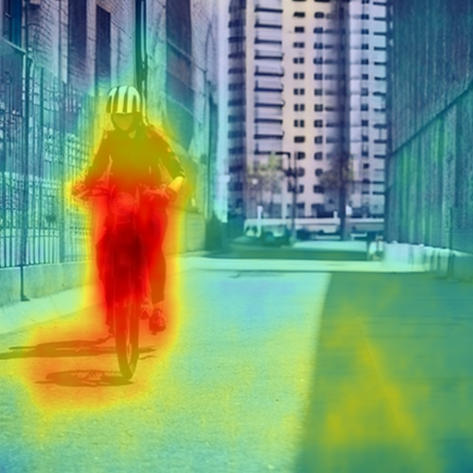
\includegraphics[width=\columnwidth]{img/4-experiments/example-linear-daam-overlay-rider.png}
   \caption{Rider}
   \label{subfig:dataset-example-rider-daam-linear}
  \end{subfigure}
  \caption[Examples of Linear DAAM-generated soft heatmaps]{Examples of Linear DAAM-generated soft heatmaps. Each subfigure displays an image for each class with the overlayed soft heatmap generated using Linear DAAM.}
  \label{fig:dataset-examples-daam-linear}
  \end{figure}


\begin{figure}
    \centering
    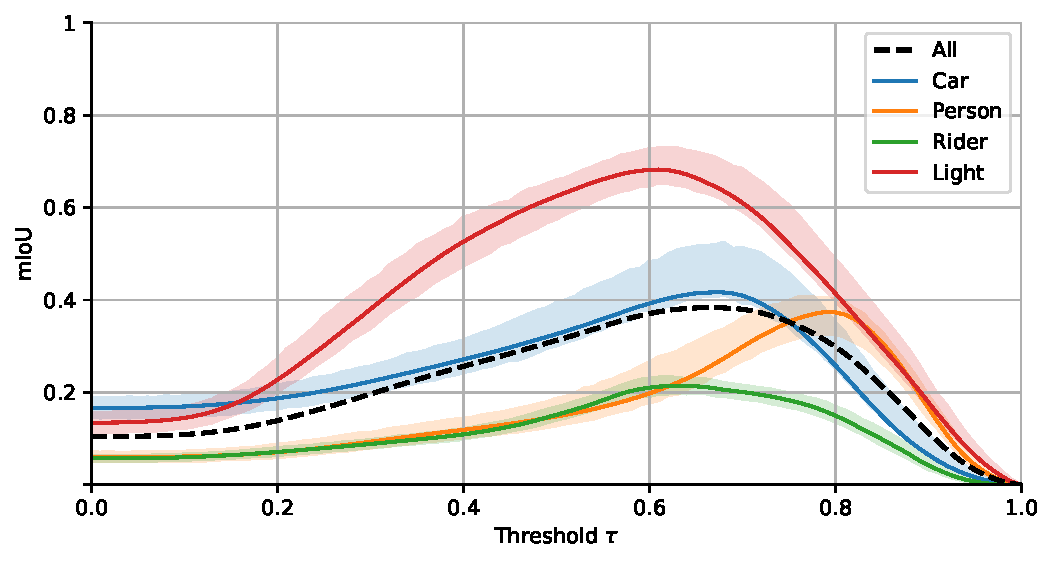
\includegraphics[width=1\columnwidth]{img/4-experiments/daam-threshold-iou-experiment-min-max-linear.pdf}
    \caption[Linear DAAM mIoU curves]{Mean Intersection over Union (mIoU) between ground truth masks and Linear DAAM heatmaps for each class at varying threshold values. The graph depicts the mIoU values for the ``car,'' ``light,'' ``person,'' and ``rider'' classes, providing insights into the pixel-wise segmentation performance. The shaded regions represent the 5th and 95th percentile values, offering a range of mIoU performance across different examples within each class.}
    \label{fig:miou-class-curves-linear}
\end{figure}


In this experiment, our objective is to assess the impact of removing the $\text{softmax}$ non-linearities in the original DAAM method \cite{DAAM} and instead utilizing Linear DAAMs (Section \ref{sec:methodology-ov-daam-linear}). It is worth noting that this experiment is not performed for the Open Vocabulary DAAM version (Section \ref{cha:methodology-ov-daam}), as evaluating it with tokens present in both the generator and the query sentence is equivalent to the original DAAM method, and thus equivalent to the previous experiment.

The $\text{softmax}$ normalization in DAAM ensures that the extracted attention is relative to the importance among different tokens in a prompt. However, by eliminating this normalization, we can construct heatmaps using a single token without the need to extract the attentions from an entire sentence, which can interfere with the attention of the target token. This provides us with more flexibility in generating ground truth based on a single word, such as the name of the object we want to segment. However, it also changes the nature of the generated heatmap as it is no longer relative to a contextual sentence.

To assess the impact of this change, we repeat the mIoU measurements on the same set of 200 dataset images, following the same threshold variation $\tau$ as in the previous experiment (Section \ref{sec:experiment-daam}). During image generation using the original text prompt ``A \textlangle token\textrangle\ in an urban environment,'' we store the attentions $\hat{h}_{t, i}$, which are then used to construct the linear soft heatmaps ${LD}^{\mathbb{R}}_X$ (see Eq. \ref{eq:daam-summing-ov-linear}). Although the proposed extension for generating Linear DAAMs allows for the evaluation of any arbitrary token, we extract the maps for the same tokens present in the prompt that generated the image to enable a meaningful comparison with the previous experiment.

Figure \ref{fig:dataset-examples-daam-linear} illustrates the resulting heatmaps for each example image. It is evident that there is a decline in performance as the generated maps exhibit more generalized attribution throughout the surroundings of the objects. For example, in Figure \ref{subfig:dataset-example-car-daam-linear} depicting an example from the "car" class, attention is now directed towards the road due to the semantic relationship between the car and that particular area of the scene. In contrast, the original method (Fig. \ref{fig:dataset-examples-daam}) produced masks that were more aligned with the actual cars. This change can be attributed to the removal of the $\text{softmax}$ with the \textlangle SOT\textrangle\ token, which typically absorbs the influence of the background areas not influenced by the primary object \cite{DAAM}. This behavior is exemplified in Figure \ref{fig:daam-example-image-1}, where the attention map of the sentence start token captures attention from the entire image background.

Analyzing Figure \ref{fig:miou-class-curves-linear}, which illustrates the threshold vs. mIoU curves, a significant reduction in performance can be observed compared to the results obtained with the original method (Fig. \ref{fig:miou-class-curves}). This can be attributed to the aforementioned behavior (Figure \ref{fig:daam-example-image-1}). Especially in the ``Car'' class, the maximum mIoU reached is 41.7, whereas with the original method we obtained 82.5.

Despite this decline in performance, these findings serve as a valuable baseline for the subsequent experiment. In the next phase, we optimize the tokens to identify the most suitable word for accurately segmenting the main object while minimizing the influence on other parts of the image. By searching for a token that precisely aligns with the desired region, we aim to mitigate this issue. Additionally, we aim to analyze how the semantic information from these optimized tokens transfers when evaluating the masks on other images that have not been specifically optimized.

\section{Text Prompt optimization}
\label{sec:experiment-optimization}


\begin{figure}
    \centering
    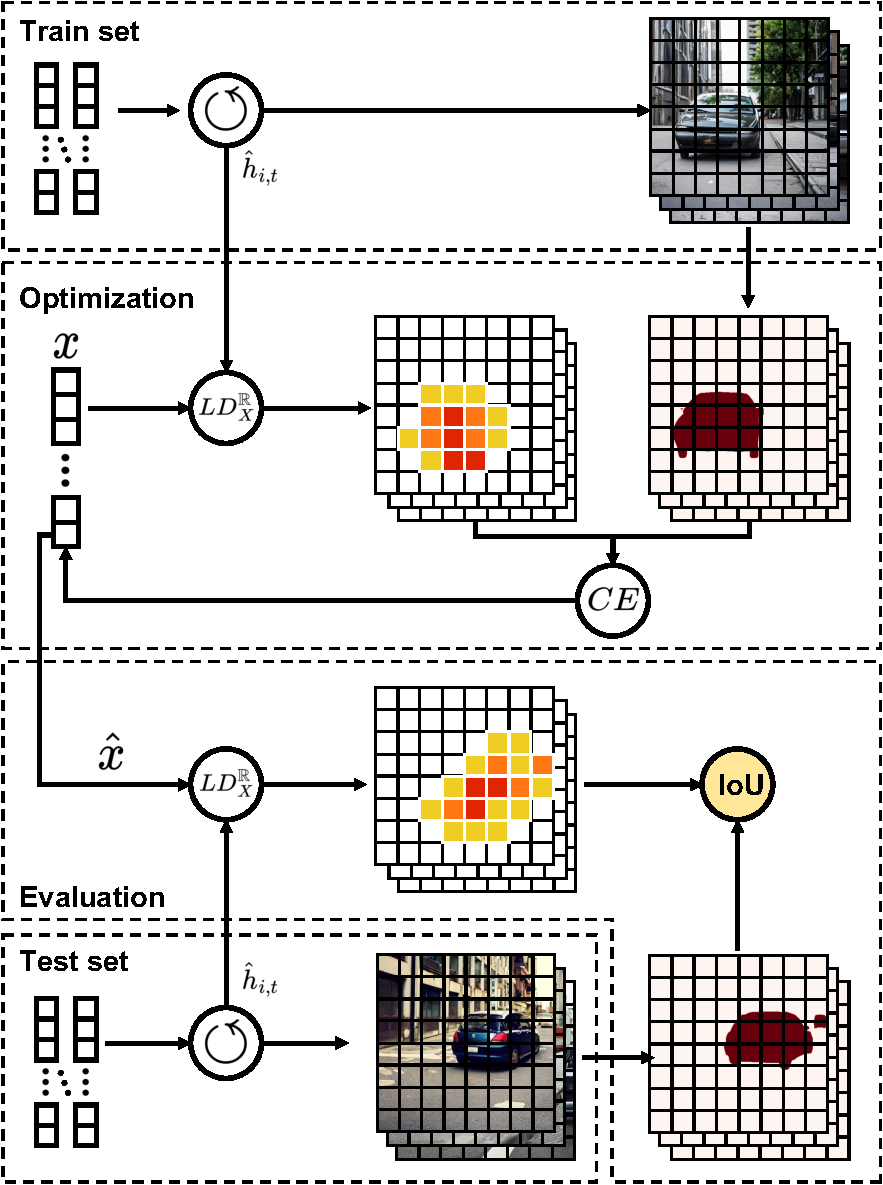
\includegraphics[width=0.98\columnwidth]{img/4-experiments/experiment-diagram.pdf}
    \caption[Experiment Design: Text Prompt Optimization for Linear DAAMs]{Experiment Design: Text Prompt Optimization for Linear DAAMs. The diagram depicts the workflow of the experiment, comprising four main steps: Train set, Optimization, Test set, and Evaluation. In the Train set phase, synthetic images are generated and manually annotated. The Optimization phase iteratively optimizes a token ``x'' to improve alignment. The Test set consists of a separate set of images. Finally, in the Evaluation phase, the optimized token is used with test attentions, and the IoU values between the test heatmaps and segmentation masks are measured.}
    \label{fig:experiment-design}
\end{figure}



\begin{figure}
\centering
  % First column
  \begin{subfigure}{0.24\columnwidth}
   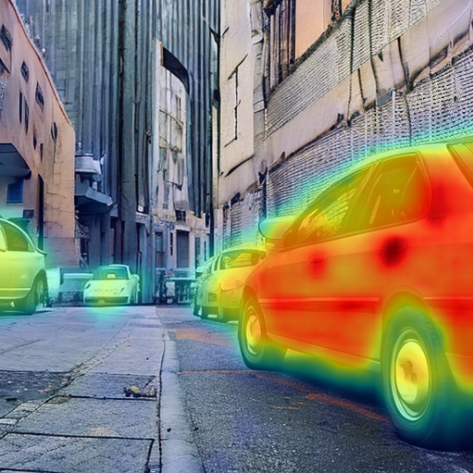
\includegraphics[width=\columnwidth]{img/4-experiments/example_daam_heatmap_car_2_epochs500.png}
   \caption{Car}
   \label{subfig:dataset-example-car-daam-linear-optimized}
  \end{subfigure}
  \begin{subfigure}{0.24\columnwidth}
   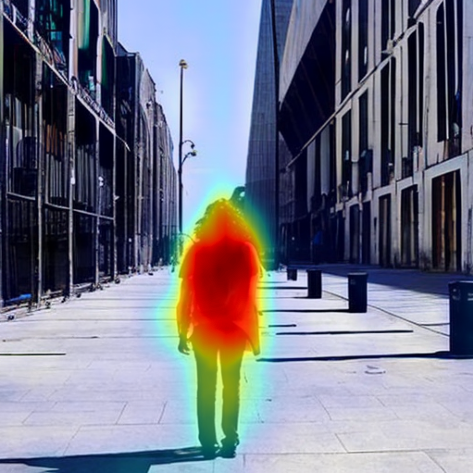
\includegraphics[width=\columnwidth]{img/4-experiments/example_daam_heatmap_person_2_epochs500.png}
   \caption{Person}
   \label{subfig:dataset-example-person-daam-linear-optimized}
  \end{subfigure}
  \begin{subfigure}{0.24\columnwidth}
   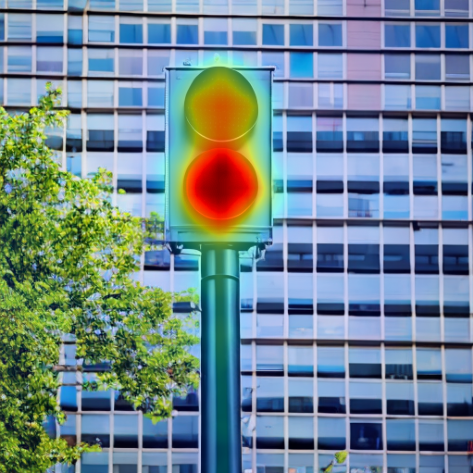
\includegraphics[width=\columnwidth]{img/4-experiments/example_daam_heatmap_light_2_epochs500.png}
   \caption{Traffic light}
   \label{subfig:dataset-example-traffic-daam-linear-optimized}
  \end{subfigure}
  \begin{subfigure}{0.24\columnwidth}
   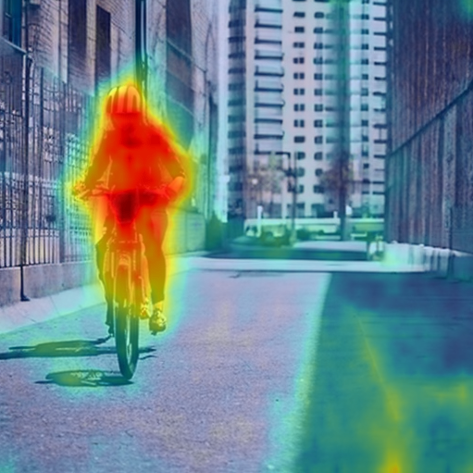
\includegraphics[width=\columnwidth]{img/4-experiments/example_daam_heatmap_rider_2_epochs500.png}
   \caption{Rider}
   \label{subfig:dataset-example-rider-daam-linear-optimized}
  \end{subfigure}
  \caption[Examples of Linear DAAM-generated soft heatmaps]{Examples of Linear DAAM-generated soft heatmaps. Each subfigure displays an image for each class with the overlayed soft heatmap generated using DAAM.}
  \label{fig:dataset-examples-daam-linear-optimized}
  \end{figure}




In this third experiment, we measure the impact of using an optimized token via DAAM for segmenting the classes. To optimize these tokens, we follow the method proposed in Section \ref{cha:methodology-ov-daam-optimization}. This optimization can be understood as "finding the most suitable word for segmenting an object," for example, representing the concept of a car $\hat{x}_{\text{car}}$ instead of using the generated attentions for the token "car".

Firstly, we conduct the optimization of the Linear DAAMs. To do this, we follow the experimental design illustrated in Figure \ref{fig:experiment-design}. We create a training set for optimization, and the remaining images are used as a test set to measure the performance curves. To evaluate the importance of the number of images used to optimize the query, we perform the experiment with 1, 2, and 5 images in the training set. For more detailed information on this optimization process, including the loss vs. epoch curves (Figure \ref{fig:apendix-loss-curves}), please refer to Appendix \ref{chap:appendix-text-prompt}.


Figure \ref{fig:dataset-examples-daam-linear-optimized} illustrates the resulting masks obtained by using the optimized tokens $\hat{x}$ with two images as the training set (different from the examples provided). The generated masks show a higher level of alignment with the targeted objects for segmentation. This is in contrast to the non-optimized Linear DAAMs (Fig. \ref{fig:dataset-examples-daam-linear}), which exhibited more dispersed attention around the objects. From a semantic perspective, this finding suggests that the optimized tokens $\hat{x}$ capture information about the objects' silhouettes while disregarding information about their surroundings.


The trend of improvement is consistently observed in the mIoU vs. threshold curves (Figure \ref{fig:miou-class-curves-linear-optimized}) when using two images to optimize the tokens.

The optimization of these tokens shows promising results in terms of their effectiveness, even with a limited number of training samples. The maximum mIoU values achieved by the curves for different training set sizes are summarized in Table \ref{tab:linear-daam-max-iou-train-test} (Figs. \ref{fig:miou-optimized-ious}). Notably, the experiment utilizing only 2 test images per class demonstrates the best performance, and in some cases, the test sets outperform the training sets. These findings suggest that the tokens $\hat{x}$ may possess semantic information that allows them to represent objects independently of their surroundings, facilitating knowledge transfer across images.



\begin{table}[ht]
\centering
\begin{tabular}{l|cc|cl|lc|}
\cline{2-7}
\multirow{2}{*}{}                   & \multicolumn{2}{c|}{1 train sample} & \multicolumn{2}{c|}{2 train samples} & \multicolumn{2}{l|}{5 train samples} \\ \cline{2-7} 
                                    & \multicolumn{1}{c|}{Train}  & Test  & \multicolumn{1}{c|}{Train}   & Test  & \multicolumn{1}{l|}{Train}   & Test  \\ \hline
\multicolumn{1}{|l|}{Car}           & \multicolumn{1}{c|}{88.4}   & 85.9  & \multicolumn{1}{c|}{86.1}    & 86.0  & \multicolumn{1}{l|}{86.3}    & \textbf{86.6}  \\
\multicolumn{1}{|l|}{Person}        & \multicolumn{1}{c|}{65.1}   & 70.0  & \multicolumn{1}{c|}{65.5}    & \textbf{71.8}  & \multicolumn{1}{l|}{65.7}    & 70.9  \\
\multicolumn{1}{|l|}{Traffic Light} & \multicolumn{1}{c|}{88.3}   & 69.7  & \multicolumn{1}{c|}{70.3}    & \textbf{72.2}  & \multicolumn{1}{l|}{70.3}    & 70.3  \\
\multicolumn{1}{|l|}{Rider}         & \multicolumn{1}{c|}{41.1}   & 38.6  & \multicolumn{1}{c|}{50.7}    & \textbf{47.8}  & \multicolumn{1}{l|}{47.4}    & 38.7  \\ \hline
\multicolumn{1}{|l|}{All}           & \multicolumn{1}{c|}{69.8}   & 63.1  & \multicolumn{1}{c|}{69.8}    & \textbf{67.3}  & \multicolumn{1}{l|}{63.6}    & 65.4  \\ \hline
\end{tabular}
\caption[Linear DAAM optimization. Comparison train and test]{Linear DAAM optimization. Comparison train and test.}
    \label{tab:linear-daam-max-iou-train-test}
\end{table}


 \begin{figure}
    \centering
    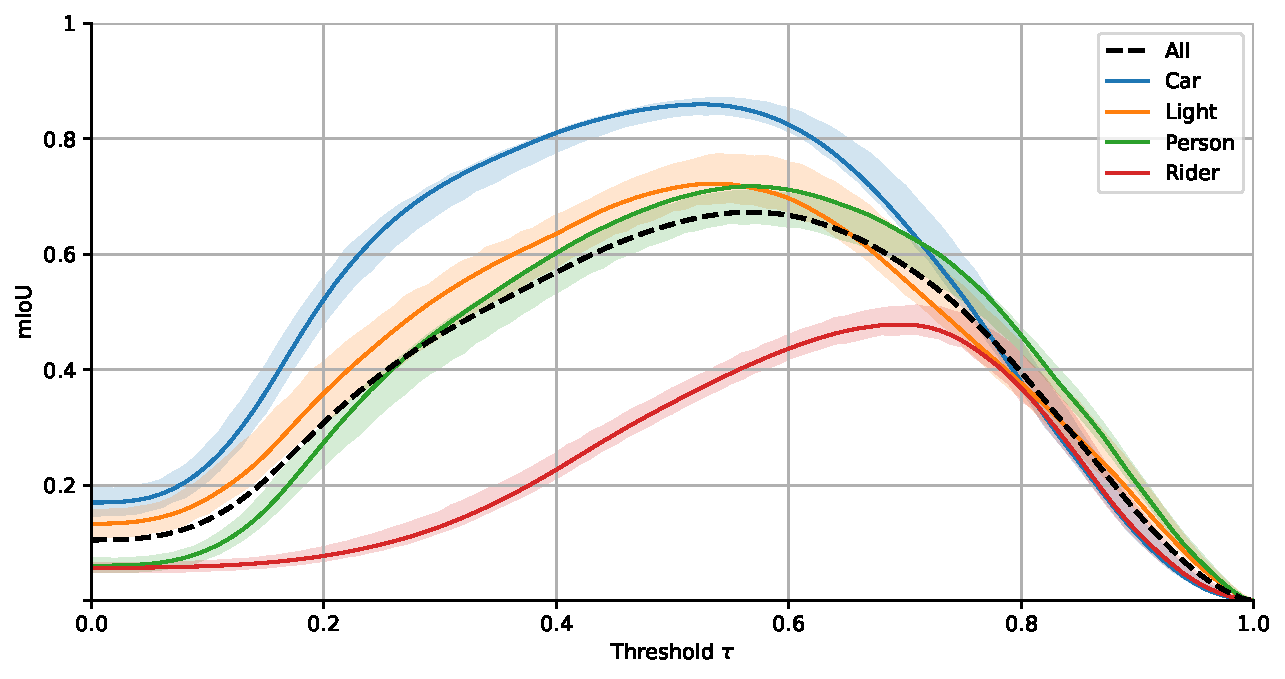
\includegraphics[width=1\columnwidth]{img/4-experiments/heatmap-optimized-iou-2-500-test-large.pdf}
    \caption[Optimized Linear DAAM mIoU curves]{Optimized Linear DAAM, mIoU vs threshold curves. Performance of the test set optimized with 2 images per class as train set.}
    \label{fig:miou-class-curves-linear-optimized}
\end{figure}

Finally, we repeated this experiment by optimizing the non-linear version of DAAM for open vocabulary (Sec. \ref{cha:methodology-ov-daam}). Unlike the linear version, in this variant, the attention is normalized across the tokens in the phrase. To perform this optimization, we followed the procedure illustrated in Figure \ref{fig:daam-general-optimization-diagram}. We used an embedding $X^\prime = [x_1, x_2]$ with two tokens. The first token was used to segment the area of the main object (e.g., car), and the second token was used to segment the background (complementary mask). The details of the optimization process can be found in Appendix \ref{chap:appendix-text-prompt}, including the loss vs. epoch curves (Fig. \ref{fig:miou-optimized-ious-daam}). The curves of mIoU vs. thresholds (Fig. \ref{fig:miou-class-curves-daam-optimized}) and examples of the masks (Fig. \ref{fig:dataset-examples-daam-optimized}) are also included in the appendix because they visually resemble the results obtained with the optimization of the linear DAAMs. This outcome indicates that optimizing a token separately or using a phrase where one token represents the background and another token represents the object produce similar results, reaffirming our hypothesis that optimizing the tokens separately converges to a token that represents the object in the text space without information about its surroundings.

In the next section, we summarize the results of the four measurements performed in the experiments: DAAM and Linear DAAM with and without optimization. This summary allows for a better understanding of the results without having to interpret the mIoU curves.

\section{Experiment Summary}
\label{sec:experiment-summary}

In summary, this chapter presents a comparison of the four measurements conducted: DAAM and Linear DAAM with and without optimization, supplemented by visual examples for qualitative comparison. To ensure an objective evaluation of segmentation performance, we utilize two metrics derived from the mIoU vs. threshold curves: the maximum IoU attained and the AUC (Area Under the Curve). The evaluations were conducted on a test set comprising 48 images per class, with the two remaining images dedicated to the prompt optimization.


The comparison of maximum mIoU values is presented in Table \ref{tab:summary-iou-results}. The results clearly indicate that the experiments using optimized tokens outperform their non-optimized counterparts for all classes. Among the optimized query versions, the non-linear variant achieves the highest maximum mIoU of 67.3 across the entire dataset, surpassing the linear version, which achieves a maximum mIoU of 66.6 for the entire dataset.

To evaluate the performance of the different versions without being affected by the chosen threshold, Table \ref{tab:summary-iou-results-auc} showcases the Area Under the Curve (AUC) instead of the maximum value. Consistently, the experiments with optimized queries outperform their non-optimized counterparts. Notably, the optimized Linear DAAM experiment achieves the highest AUC of 39.5 for the entire dataset, primarily driven by its strong performance in the "Person" class.

For a qualitative comparison of these results, Figure \ref{fig:final-examples} presents several examples from each class, illustrating a consistent pattern observed in the tables. In the ``traffic light'' class, all versions exhibit similar performance, with masks centered around the traffic lights. However, in the ``Person'' and ``Car'' classes, the non-optimized Linear DAAMs amplify the scattered attention observed in the original DAAM version. On the other hand, in the ``Rider'' case, where the attention naturally aligns with the bicycle, the optimization successfully focuses the attention on the rider, aligning with the intended ground truth.

These preliminary findings provide support for the hypothesis that by ``searching'' for a more suitable word to describe an object, it is feasible to guide the attention of a text-to-image LDM and extract segmentation masks for specific object classes. In the next chapter, we present our conclusions and initiate a discussion on potential directions for further investigation in this study, as well as explore potential applications in various tasks.


\begin{table}[ht]
\centering
\begin{tabular}{l|cc|cc|}
\cline{2-5}
\multirow{2}{*}{}                   & \multicolumn{2}{c|}{Non-Optimized} & \multicolumn{2}{c|}{Optimized}             \\ \cline{2-5} 
                                    & \multicolumn{1}{c|}{DAAM}  & LDAAM & \multicolumn{1}{c|}{DAAM}          & LDAAM \\ \hline
\multicolumn{1}{|l|}{Car}           & \multicolumn{1}{c|}{82.5}  & 41.7  & \multicolumn{1}{c|}{\textbf{86.0}} & 85.8  \\
\multicolumn{1}{|l|}{Person}        & \multicolumn{1}{c|}{36.2}  & 37.4  & \multicolumn{1}{c|}{\textbf{71.6}} & 71.3  \\
\multicolumn{1}{|l|}{Traffic Light} & \multicolumn{1}{c|}{71.1}  & 68.2  & \multicolumn{1}{c|}{\textbf{72.5}} & 72.3  \\
\multicolumn{1}{|l|}{Rider}         & \multicolumn{1}{c|}{31.0}  & 21.3  & \multicolumn{1}{c|}{\textbf{47.6}} & 43.1  \\ \hline
\multicolumn{1}{|l|}{All}           & \multicolumn{1}{c|}{53.2}  & 38.3  & \multicolumn{1}{c|}{\textbf{67.3}} & 66.6  \\ \hline
\end{tabular}
\caption[Summary of experiments: mIoU]{Summary of experiments: maximun mIoU}
    \label{tab:summary-iou-results}
\end{table}



\begin{table}[ht]
\centering
\begin{tabular}{l|cc|cc|}
\cline{2-5}
\multirow{2}{*}{}                   & \multicolumn{2}{c|}{Non-Optimized} & \multicolumn{2}{c|}{Optimized}                     \\ \cline{2-5} 
                                    & \multicolumn{1}{c|}{DAAM}  & LDAAM & \multicolumn{1}{c|}{DAAM}          & LDAAM         \\ \hline
\multicolumn{1}{|l|}{Car}           & \multicolumn{1}{c|}{39.7}  & 23.7  & \multicolumn{1}{c|}{\textbf{51.6}} & 51.5          \\
\multicolumn{1}{|l|}{Person}        & \multicolumn{1}{c|}{13.8}  & 15.4  & \multicolumn{1}{c|}{36.6}          & \textbf{41.3} \\
\multicolumn{1}{|l|}{Traffic Light} & \multicolumn{1}{c|}{43,3}  & 38.3  & \multicolumn{1}{c|}{\textbf{42.8}} & 42.7          \\
\multicolumn{1}{|l|}{Rider}         & \multicolumn{1}{c|}{15.6}  & 11.0  & \multicolumn{1}{c|}{\textbf{23.5}} & 22.5          \\ \hline
\multicolumn{1}{|l|}{All}           & \multicolumn{1}{c|}{28.1}  & 22.1  & \multicolumn{1}{c|}{38.6}          & \textbf{39.5} \\ \hline
\end{tabular}
\caption[Summary of experiments: AUC]{Summary of experiments: AUC}
    \label{tab:summary-iou-results-auc}
\end{table}




\begin{figure}
    \centering
    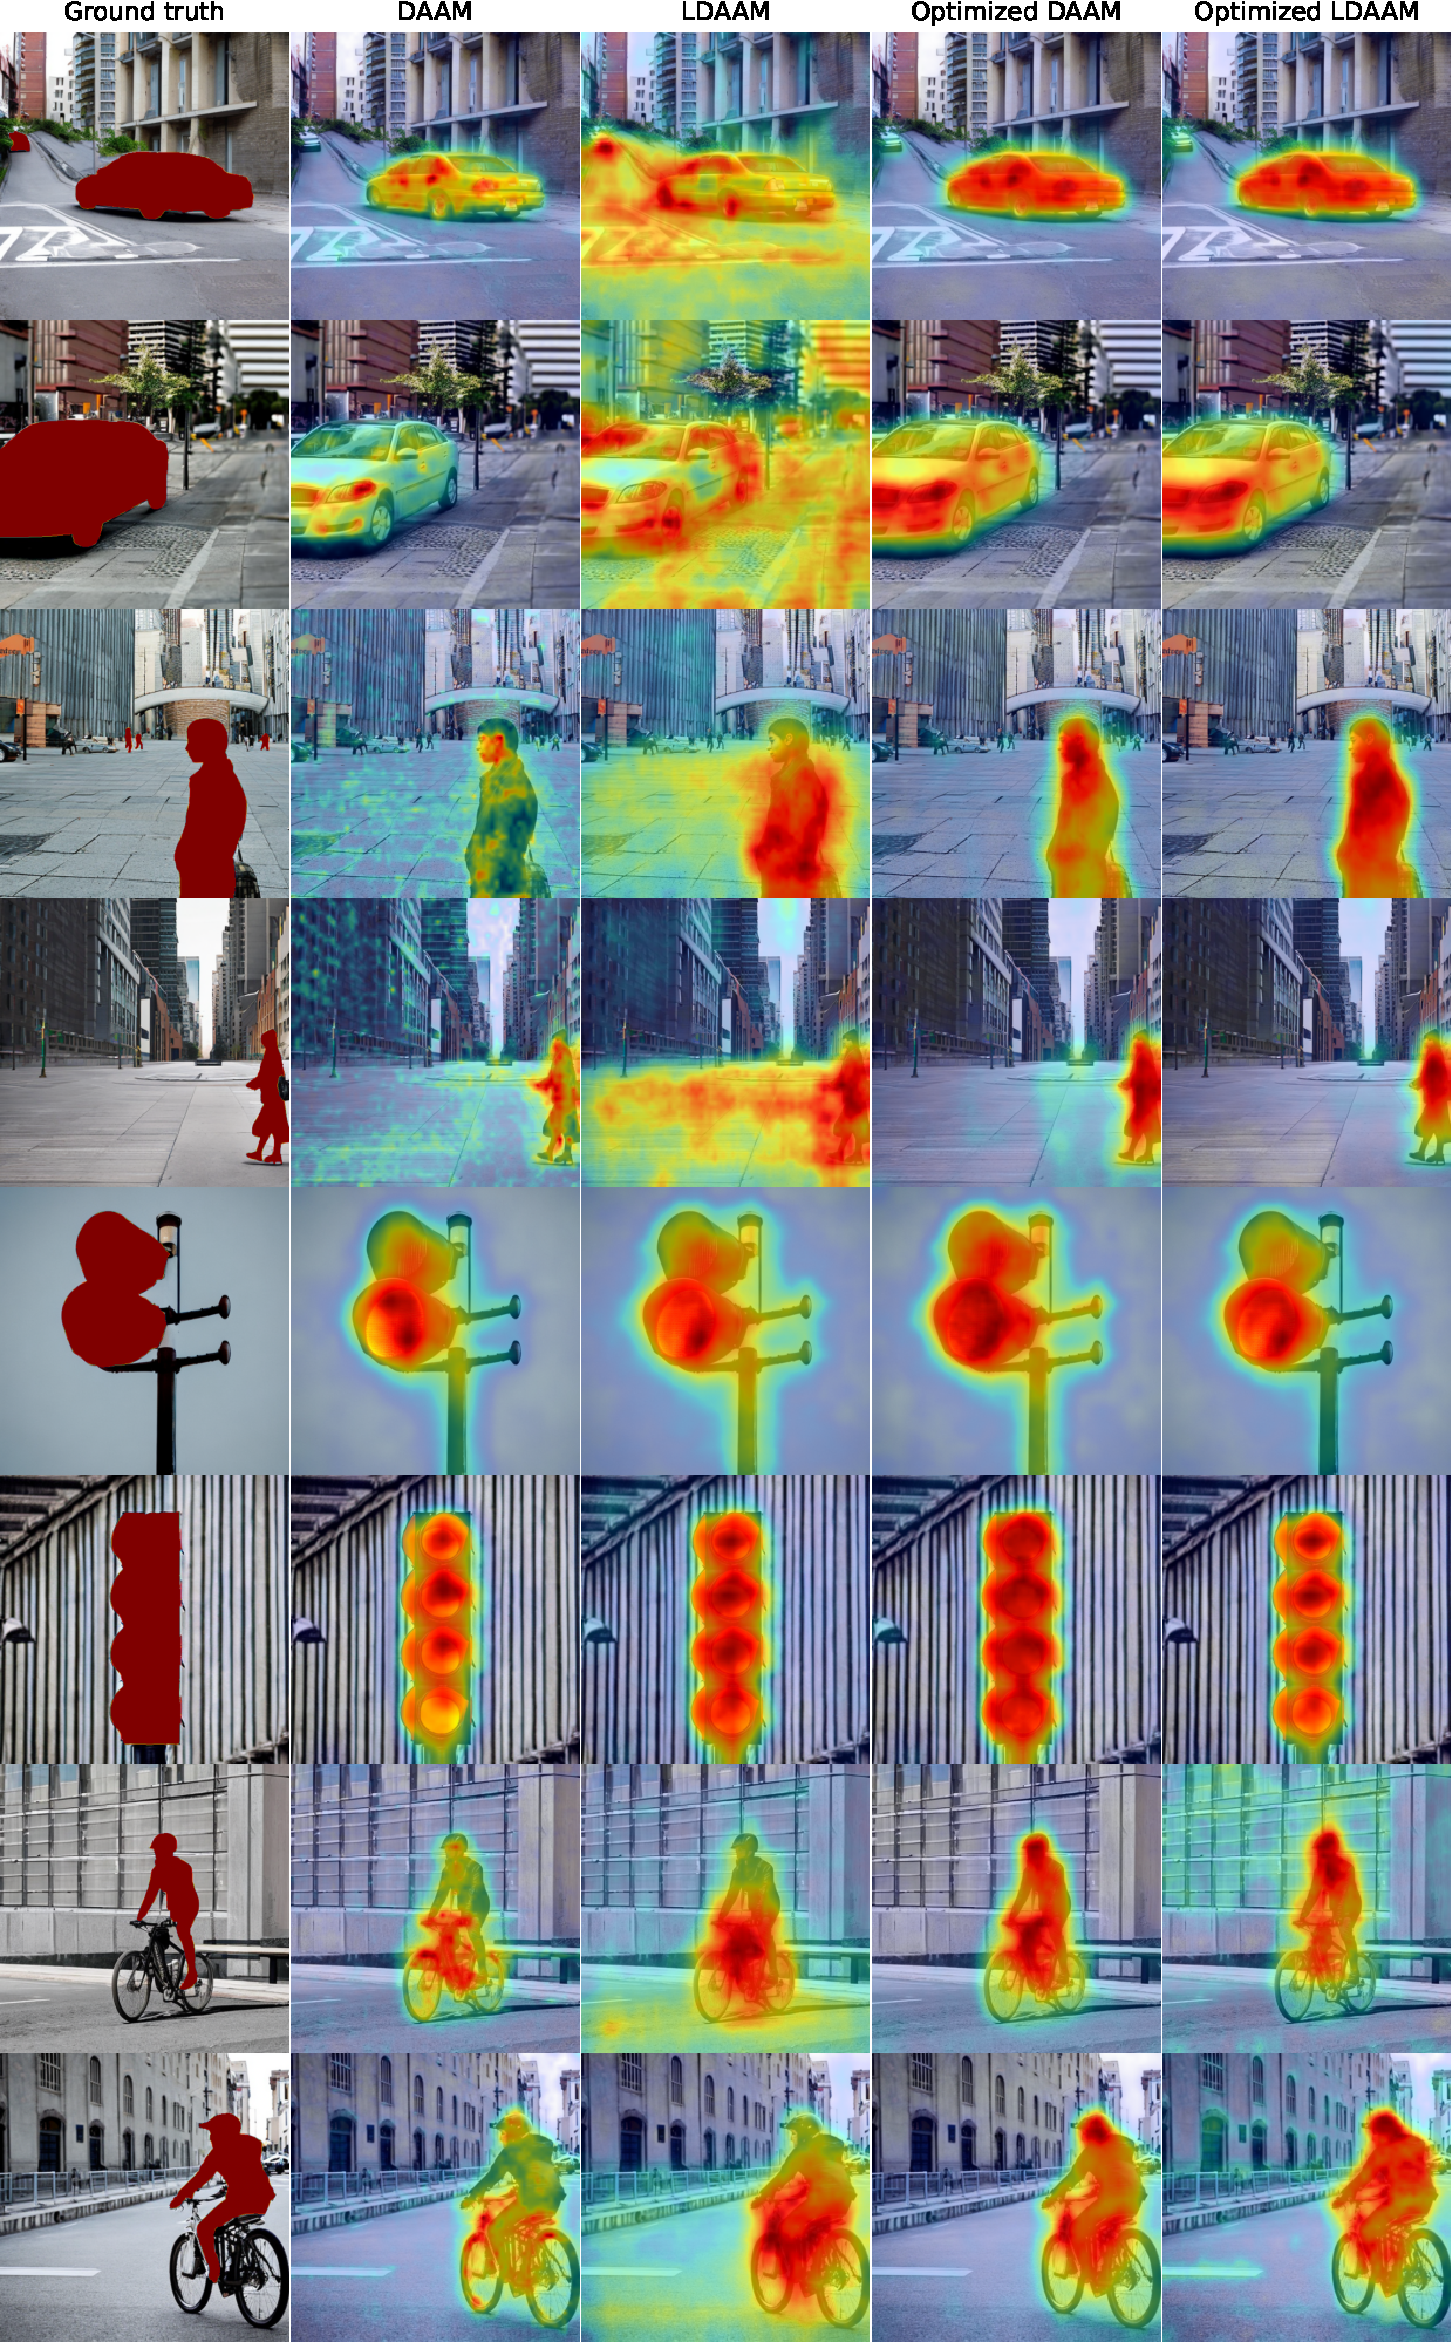
\includegraphics[width=0.93\columnwidth]{img/4-experiments/final_examples_2.pdf}
   \caption[Experiments examples]{Experiments examples. By columns: Ground truth, DAAM, Linear DAAM, DAAM with prompt optimized, Linear DAAM Optimized.}
    \label{fig:final-examples}
\end{figure}
